\documentclass[17pt,sans,mathserif]{beamer}

\usetheme{ddb}
\setbeamertemplate{navigation symbols}{}

\usepackage[absolute,overlay]{textpos}
\setlength{\TPHorizModule}{1pt}
\setlength{\TPVertModule}{1pt}
\usepackage{sgamevar}
\usepackage{tikz}

\newenvironment{framebg}[1]
{
  \begingroup
    \usebackgroundtemplate{\includegraphics[width=\paperwidth,height=\paperheight]{#1}}
    \begin{frame}
}
{
    \end{frame}
  \endgroup
}

\newcommand{\switchnormaltextcolor}[1]{
  \setbeamercolor{normal text}{use={#1},fg={#1.fg}, bg={#1.bg}}
  \usebeamercolor[fg]{#1}
}
\newenvironment{framestruct}
{
  \begingroup
  \switchnormaltextcolor{structural frame}
    \begin{frame}
}
{
    \end{frame}
  \endgroup
}

\newcommand{\framestructtitle}[1]{
  \begin{center}
    \Huge
    \textbf{#1}
  \end{center}
}

\begin{document}

% -*- TeX-master: "presentation"; TeX-command-default: "SCons"; -*-

\begin{framebg}{images/game_theory.jpg}
\end{framebg}

\begin{frame}
  \frametitle{Previously in \emph{Game Theory}}

  \pause
  \begin{itemize}
  \item decision makers:
    \begin{itemize}
    \item choices
    \item preferences
    \end{itemize}
  \pause
  \item solution concepts:
    \begin{itemize}
    \item best response
    \item Nash equilibrium
    \end{itemize}
  \end{itemize}
\end{frame}

\begin{frame}
  \frametitle{Rock, paper, scissors}
  \pause
  \begin{game}{3}{3}
      \> $R$     \> $P$     \> $S$     \\
    $R$ \> $0, 0$  \> $-1, 1$ \> $1, -1$ \\
    $P$ \> $1, -1$ \> $0, 0$  \> $-1, 1$ \\
    $S$ \> $-1, 1$ \> $1, -1$ \> $0, 0$
  \end{game}

\end{frame}

\begin{framestruct}
  \Large
  \textbf{Learning in games}
  \bigskip
  \pause

  \textbf{Repeated games}
\end{framestruct}

% -*- TeX-master: "presentation"; TeX-command-default: "SCons"; -*-

\begin{framestruct}
\framestructtitle{Learning in games}
\end{framestruct}

\begin{frame}
  \frametitle{Best Response learning}

  \begin{enumerate}
  \pause \item Guess what the opponent(s) will play
  \pause \item Play a Best Response to that guess
  \pause \item Observe the play
  \pause \item Update the guess
  \end{enumerate}

\end{frame}

\begin{frame}
  \frametitle{BR learning: Cournot dynamics}
  \pause
  Guess = last action played
  \pause

  \begin{game}{2}{2}
      \> $C$     \> $D$    \\
    $C$ \> $2, 2$  \> $-1, 3$\\
    $D$ \> $3, -1$ \> $0, 0$ \\
  \end{game}
  \pause

  \begin{game}{3}{3}
      \> $R$     \> $P$     \> $S$     \\
    $R$ \> $0, 0$  \> $-1, 1$ \> $1, -1$ \\
    $P$ \> $1, -1$ \> $0, 0$  \> $-1, 1$ \\
    $S$ \> $-1, 1$ \> $1, -1$ \> $0, 0$
  \end{game}

\end{frame}

\begin{frame}
  \frametitle{BR learning: Fictitious play}
  \pause
  Guess = empirical distribution of play
  \pause
  \begin{game}{3}{3}
      \> $R$     \> $P$     \> $S$     \\
    $R$ \> $0, 0$  \> $-1, 1$ \> $1, -1$ \\
    $P$ \> $1, -1$ \> $0, 0$  \> $-1, 1$ \\
    $S$ \> $-1, 1$ \> $1, -1$ \> $0, 0$
  \end{game}
  \pause
  \begin{game}{3}{3}
      \> $L$    \> $C$    \> $R$    \\
    $U$ \> $0, 0$ \> $0, 1$ \> $1, 0$ \\
    $M$ \> $1, 0$ \> $0, 0$ \> $0, 1$ \\
    $D$ \> $0, 1$ \> $1, 0$ \> $0, 0$
  \end{game}
\end{frame}

\begin{frame}
  \frametitle{Evolutionary learning}
  \pause
  Action set: $A$

  Utility function: $u$

  \pause
  \bigskip
  $p \in \Delta(A), k \in A$

  $\dot{p_k} = p_k\left(u(k, p) - u(p, p)\right)$
\end{frame}

\begin{frame}
  \frametitle{Battle of the Sexes}

  \pause
  \begin{game}{2}{2}
      \> $O$     \> $F$    \\
    $O$ \> $3, 2$  \> $0, 0$ \\
    $F$ \> $0, 0$  \> $2, 3$ \\
  \end{game}
\end{frame}

\begin{frame}
  \frametitle{Correlated equilibrium (CE)}
  \pause
  $a^* \in A = \prod_iA_i$ is a NE:
  \[\forall i, \forall a'_i, u_i(a_i^*, a_{-i}^*) \ge u_i(a_i', a_{-i}^*)\]

  \pause
  $\alpha \in \prod_i\Delta(A_i)$ is a NE: $\forall i, \forall a_i, \forall a'_i,$
  \[\sum_{a_{-i}} u_i(a_i, a_{-i}) \alpha(a) \ge
  \sum_{a_{-i}} u_i(a_i',
  a_{-i}) \alpha(a) \]

  \pause
  $\pi \in \Delta(A)$ is a CE: $\forall i, \forall a_i, \forall a'_i,$
  \[\sum_{a_{-i}} u_i(a_i, a_{-i}) \pi(a) \ge
  \sum_{a_{-i}} u_i(a_i', a_{-i}) \pi(a) \]
\end{frame}

\begin{frame}
  \frametitle{No regret learning}
  \pause
  \[u_i(k, a_{-i}) - u_i(j, a_{-i})\]
  \pause
  \[R^i_{jk}(t) = \sum_{\tau = 0: a_i(\tau) = j}^t u_i(k, a_{-i}(\tau)) - u_i(j,
  a_{-i}(\tau))\]
  \pause
  Regret matching converges to the correlated equilibria set.
\end{frame}

\begin{framestruct}
  \frametitle{Learning in games}

  \begin{itemize}
  \pause \item Best response
  \pause \item Replicator dynamics
  \pause \item No regret
  \end{itemize}

\end{framestruct}

% -*- TeX-master: "presentation"; TeX-command-default: "SCons"; -*-

\begin{framestruct}
  \framestructtitle{Repeated games}
\end{framestruct}

\begin{frame}
  \frametitle{Markov Decision Process (MDP)}
  \pause
  state space $X$

  action space $U$

  transition $P:X\times U \to \Delta(X)$

  reward $r:X \times U \to \mathbb{R}$

  discount factor $\delta \in [0,1]$


  \pause
  \bigskip
  \[U(x(\cdot), u(\cdot)) = \sum_{t=0}^{+\infty} \delta^t r(x(t), u(t))\]
\end{frame}

\begin{frame}
  \frametitle{MDP (continued)}
  history $\mathcal{H} \in \prod (X,U)$

  policy $\pi: \mathcal{H} \to \Delta(U)$

  \pause
  $V^\pi(x_0) = \mathbb{E}_{\pi}\left[U(x(\cdot), u(\cdot))\right]$

  \pause
  \[V(x_0) = \max_{\pi} V^\pi(x_0)\]

\end{frame}

\begin{frame}
  \frametitle{Principle of Optimality}

  Bellman's equation:
  \[V(x_0) = \max_{u_0} \left[r(x_0, u_0) + \delta V(P(x_0, u_0))\right]\]
\end{frame}

\begin{frame}
  \frametitle{Dynamic Programming}

  Solving the MDP:
  \begin{itemize}
  \pause \item knowing $P$: value iteration
  \pause \item not knowing $P$: online learning
  \end{itemize}

\end{frame}

\begin{frame}
  \frametitle{Repeated game}
  \pause
  Game $(\mathcal{I}, \prod_i A_i, \prod_i u_i)$

  \pause
  Discount factor $\delta$
  \[U_i(a(\cdot)) = \sum_{t=0}^{+\infty} \delta^t u_i(a(t))\]

  \pause
  Strategy $\sigma: \mathcal{H} \to \prod_i \Delta(A_ix)$
  \[V_i(\sigma) = \mathbb{E}_{\sigma}\left[U_i(a(\cdot))\right]\]
\end{frame}

\begin{frame}
  \frametitle{Nash equilibrium}

  Player $i$:
  \begin{itemize}
  \item choices $\sigma_i$
  \item utility $V_i$
  \end{itemize}

  \pause
  Nash equilibrium is not strong enough!
  (Explanation on the whiteboard {\Huge $\Rightarrow$})
\end{frame}

\begin{frame}
  \frametitle{Information structure}

  \pause
  \begin{itemize}
  \item perfect
  \item imperfect
  \end{itemize}

  \pause
  \begin{itemize}
  \item public
  \item private (beliefs)
  \end{itemize}

\end{frame}

\begin{frame}
  \frametitle{Folk theorem}

  Any feasible, strictly individually rational payoff can be sustained by a
  sequentially rational equilibrium.

  \pause
  \bigskip
  Holy grail for repeated games.
\end{frame}

\begin{frame}
  \begin{figure}
  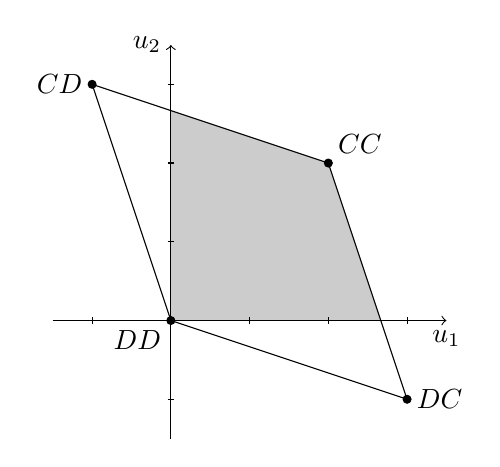
\begin{tikzpicture}[scale=1,
                      axes/.style=,
                      payoffs/.style=,
                      feasible/.style={opacity=0.2}]
    % -*- TeX-master: "article"; TeX-command-default: "SCons"; -*-

% Defining the axes
\def\stepmin{-1}
\def\stepmax{3}
\def\stepextra{0.5}
\def\ticklen{0.04}
\coordinate (x min) at (\stepmin - \stepextra, 0) {};
\coordinate (y min) at (0, \stepmin -\stepextra) {};
\coordinate (x max) at  (\stepmax + \stepextra, 0) {};
\coordinate (y max) at  (0, \stepmax + \stepextra) {};

% Defining the payoffs
\coordinate (CC) at  (2, 2) {};
\coordinate (CD) at (-1, 3) {};
\coordinate (DC) at (3, -1) {};
\coordinate (DD) at  (0, 0) {};
\coordinate (minimax) at (0,0) {};

\begin{scope}[axes]
  % Drawing the axes
  \draw [->] (x min) -- (x max);
  \draw [->] (y min) -- (y max);

  % Drawing the ticks
  \foreach \step in {\stepmin, ..., \stepmax}
  {
    \draw (-\ticklen, \step) -- (\ticklen, \step);
    \draw (\step, -\ticklen) -- (\step, \ticklen);
  }

  % Labelling the axes
  \node [below] at (x max) {$u_1$};
  \node [left] at (y max) {$u_2$};
\end{scope}

\begin{scope}[payoffs]
  % Drawing the feasible, rational payoffs
  \begin{scope}[feasible]
    \clip <5> (minimax) -- (y max) -| (x max);
    \fill <4-> (CC) -- (CD) -- (DD) -- (DC) -- cycle;
  \end{scope}

  % Drawing the payoff envelope
  \draw <4-> (CC) -- (CD) -- (DD) -- (DC) -- cycle;

  \filldraw <3-> (CC) circle (0.05);
  \filldraw <3-> (CD) circle (0.05);
  \filldraw <2-> (DC) circle (0.05);
  \filldraw <3-> (DD) circle (0.05);

  % Labelling the pure strategies payoffs
  \node <3-> [above right] at (CC) {$CC$};
  \node <3-> [below left] at (DD) {$DD$};
  \visible <2-> {\node [right] at (DC) {$DC$};}
  \visible <3-> {\node [left] at (CD) {$CD$};}
\end{scope}

  \end{tikzpicture}
  \end{figure}
\end{frame}

\begin{framestruct}
  \framestructtitle{Research}
\end{framestruct}

\begin{frame}
  \frametitle{Weakly belief-free equilibria}

  Characterization of repeated games with correlated equilibria.
\end{frame}


\begin{framestruct}
  \frametitle{Repeated games}

  \begin{itemize}
  \pause \item Dynamic programming
  \pause \item Repeated games
  \pause \item Folk theorem
  \end{itemize}

\end{framestruct}

% -*- TeX-master: "presentation"; TeX-command-default: "SCons"; -*-

\begin{framestruct}
  \Large
  \textbf{Learning in games}
  \bigskip
  \pause

  \textbf{Repeated games}
\end{framestruct}

\begin{framestruct}
  \textbf{\Huge Questions, \\ \bigskip Comments}
\end{framestruct}

\end{document}
